\documentclass[12pt,a4]{article}

\usepackage{graphicx,subfigure,amsmath,amssymb,amsthm, boxedminipage,xcolor,float,enumerate,geometry}
\usepackage[lined,boxed]{algorithm2e}
\geometry{left=3cm,right=3cm,top=1.5cm,bottom=3.5cm}
\date{}

\title{
	Assignment 8\\
	\vspace{3mm}
	{\normalsize 516030910259 \textbf{Xinpeng Liu}}
}
\begin {document}
	\maketitle
	\paragraph{8.3}
	\begin{center}
	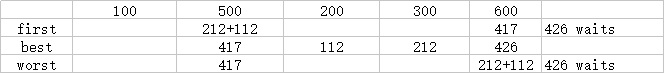
\includegraphics[width=\textwidth]{1.jpg}
	\end{center}
	Best-fit algorithm makes the most efficient use of memory.
	\paragraph{8.7}.
	Segmentation requires more space for translations structure. Every segmentation is corresponding to two registers: base and limit, while every page is corresponding to only one register storing the corresponding frame. 
	\paragraph{8.9}
	\begin{enumerate}[a.]
		\item 400 nanoseconds.
		\item 200*0.75+400*0.25=250 nanoseconds
	\end{enumerate}
	\paragraph{8.12}
	\begin{enumerate}[a.]
		\item 649
		\item 2310
		\item No such address.
		\item 1727
		\item No such address.
	\end{enumerate}
\end {document}